% Summary of hanson2025: Tier-based strict locality and the typology of agreement

\begin{abstract}
Tier-based Strict Locality captures Case-sensitive Agreement, Complementizer Agreement, Multiple Agreement, Chain Agreement, invisibility, and blocking.

Key empirical facts to explain:

\begin{itemize}
  \item Hindi-Urdu verbs always agree with the highest nominative
  \begin{itemize}
    \item Project only D[nom]
  \end{itemize}
  \item Nepali verbs always agree with the highest nominative or ergative
  \begin{itemize}
    \item Project only D[nom] and D[erg]
  \end{itemize}
  \item Icelandic verbs agree with nominatives, and dative subjects don’t block agreement with nominative objects, but dative goals alongside expletive subjects do
  \begin{itemize}
    \item Project all D[nom], plus all D[dat] that don’t have EPP
    \item \#me this seems like it could be a movement thing
  \end{itemize}
  \item Subject-verb agreement is usually downwards-looking
  \item Negative Concord is upwards-looking
  \item Case Concord is upwards-looking if case goes on D
  \item West Flemish complementizers agree downward for number with embedded subjects
  \item Lubukusu complementizers (sometimes) agree upward for noun class with higher subject
  \item Diercks 2013 argues that the matrix subject binds an operator in specCP which agrees locally with C, calling this Indirect Agreement
  \begin{itemize}
    \item Agreement is strictly subject-oriented; intervening DPs are ignored
    \item In subject questions the verb follows a reduced agreement pattern, but complementizer agreement is normal
    \item Lubukusu also has hyperraising, which makes complementizer agreement absent
  \end{itemize}
\end{itemize}

Other thoughts:

\begin{itemize}
  \item previous parallels between agreement and phonological Harmony: Nevins 2010
  \item How do we represent the difference between C, which blocks wh-movement cross-linguistically (if true), and things which only sometimes block wh-movement?
\end{itemize}

Key things to explain that it explicitly does not:

\begin{itemize}
  \item subfeatures of phi acting independently (need multiple tiers for that)
  \item a single predicate agreeing with multiple DPs (but see Deal on interaction/satisfaction theory)
  \item Optionality in Agreement: English expletive agreement
  \begin{itemize}
    \item Could use multiple grammars (Kroch 1989) or Interaction-Satisfaction Theory
  \end{itemize}
  \item movement feeding subsequent operations
  \item Implicational hierarchies like the fact that you can first only agree with nominative, then dependent cases (acc, erg), and then oblique (dat) (Bobaljik 2008)
  \begin{itemize}
    \item Extragrammatical factors, monotonicity effects like in Graf 2020
    \item Formalizing it more than this would still leave the question of why it’s this way
    \item \#me but it would clearly still help to have a good formalism; to know how these rules might be represented in existing symbolic languages
  \end{itemize}
\end{itemize}
\end{abstract}

\section*{More Notes}

draws on Bobaljik 2008, Deal 2015, Keine 2019, etc.

previous parallel between Agreement and Harmony: Nevins 2010

\subsection*{1 me questions}

\begin{enumerate}
  \item How do we represent the difference between C, which blocks wh-movement cross-linguistically (does it?), and things which only sometimes block
\end{enumerate}

\subsection*{types of agreement}

\begin{center}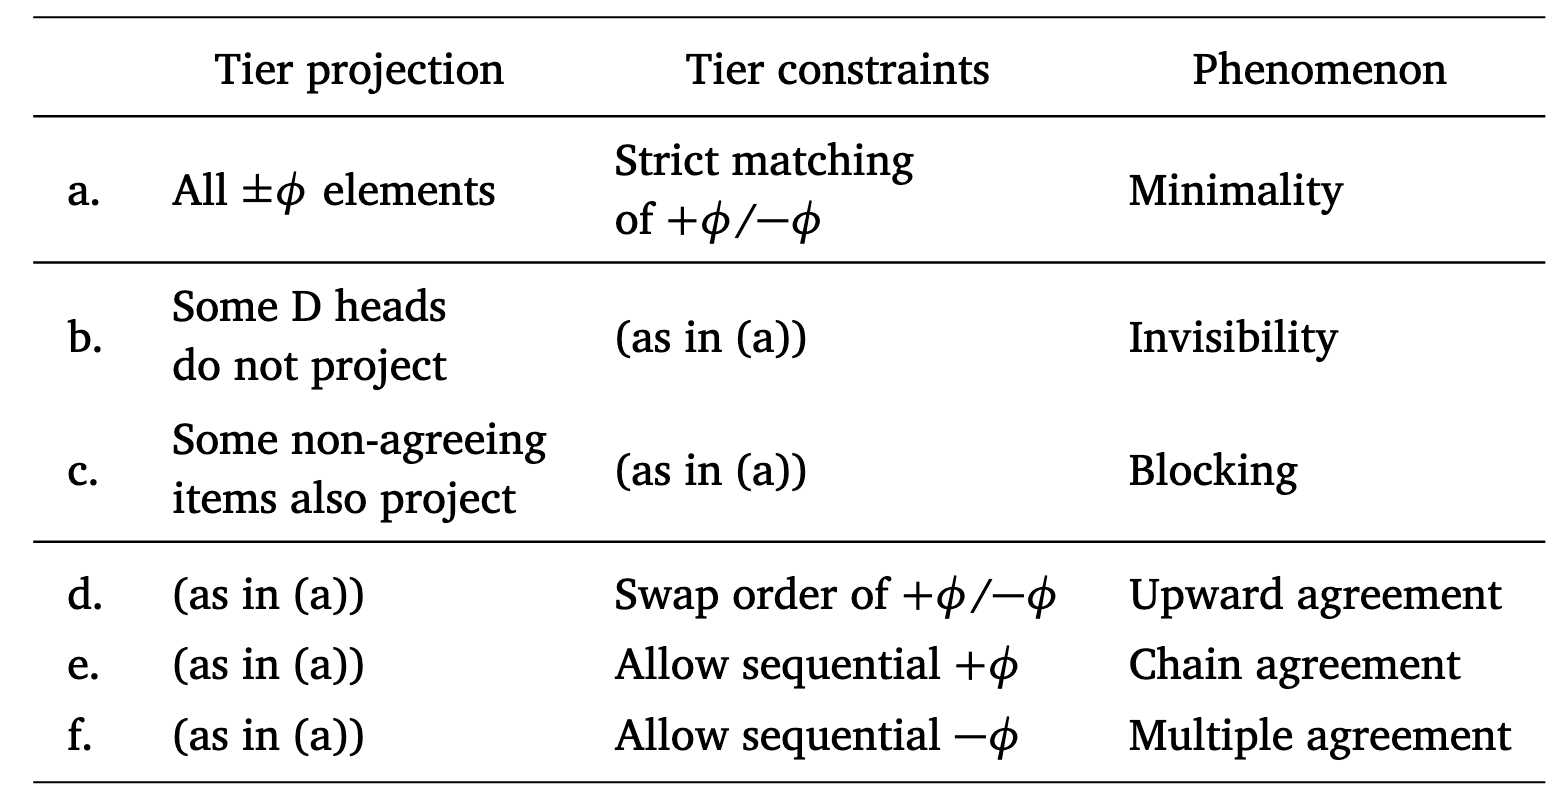
\includegraphics[width=0.68\linewidth]{images/pasted-20260922055710.png}\end{center}

not exhaustive; focuses on Case-Sensitive Agreement and Complementizer Agreement

\begin{itemize}
  \item do not treat patterns in which:
  \begin{itemize}
    \item subfeatures of phi act independently; these need MTSLs.
    \item a single predicate agrees with multiple DPs; \textit{for reasons in s2.4}
    \begin{itemize}
      \item but sketch how this could be done with Interaction-Satisfaction Theory (Deal 2015)
    \end{itemize}
  \end{itemize}
\end{itemize}

Present model struggles with movement feeding subsequent operations: s3.2

\subsubsection*{2.1 variation in set of elements projected onto the tier}

\paragraph*{2.1.1 Hindi (agree with highest nominative: project on case)}

Hindi:

\begin{itemize}
  \item in perfective clauses, the subject gets ergative
  \item the verb always agrees with the highest nominative
\end{itemize}

Solution:

\begin{itemize}
  \item project only nominative DPs onto the tier
\end{itemize}
\textit{assume case is present and available to condition on; see Preminger 2014 and Bobaljik 2008}

\begin{center}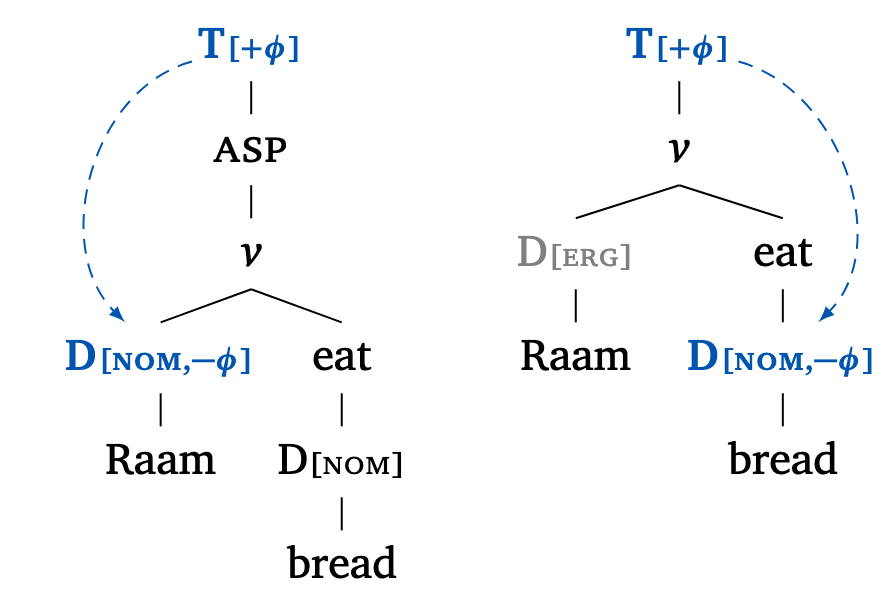
\includegraphics[width=0.48\linewidth]{images/pasted-20260922055737.png}\end{center}

\begin{center}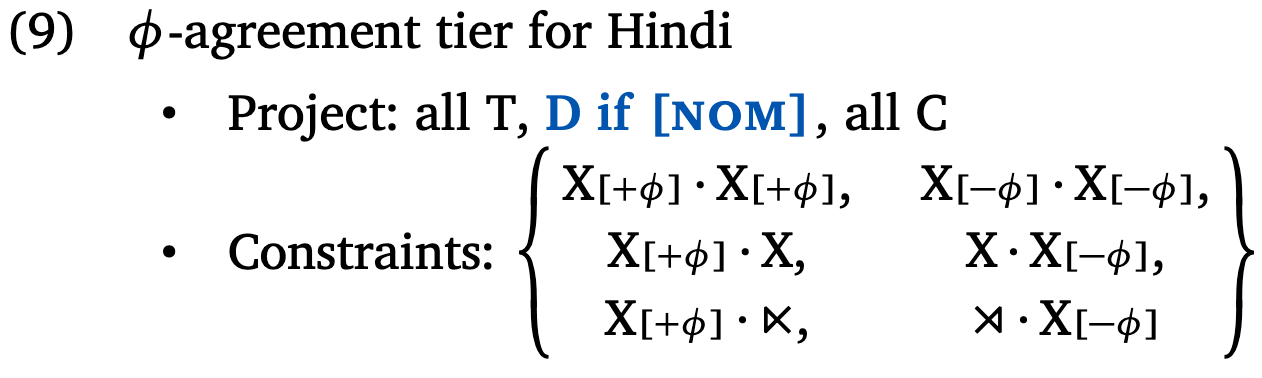
\includegraphics[width=0.53\linewidth]{images/pasted-20260922055744.png}\end{center}

\paragraph*{2.1.2 Nepali (agree with highest nominative/ergative)}

same as Hindi, except

project nominative and ergative DPs, but not dative DPs

\begin{itemize}
  \item there's a hierarchy cross-linguistically, from agreeing with unmarked case (nominative) to dependent cases (accusative, ergative) to oblique cases (dative) Bobaljik 2008
  \item these kind of implicational hierarchies should be attributed to extragrammatical factors, part of a larger class of monotonicity effects, see Graf 2020 - so it's fine that TSL doesn't rule out the bad ones (plus if you formalized it you still have to ask why it is this way)
\end{itemize}

\paragraph*{2.1.3 Icelandic (datives sometimes block but never agree: project on EPP)}

Dative Intervention

No blocking in simple transitive:

\begin{center}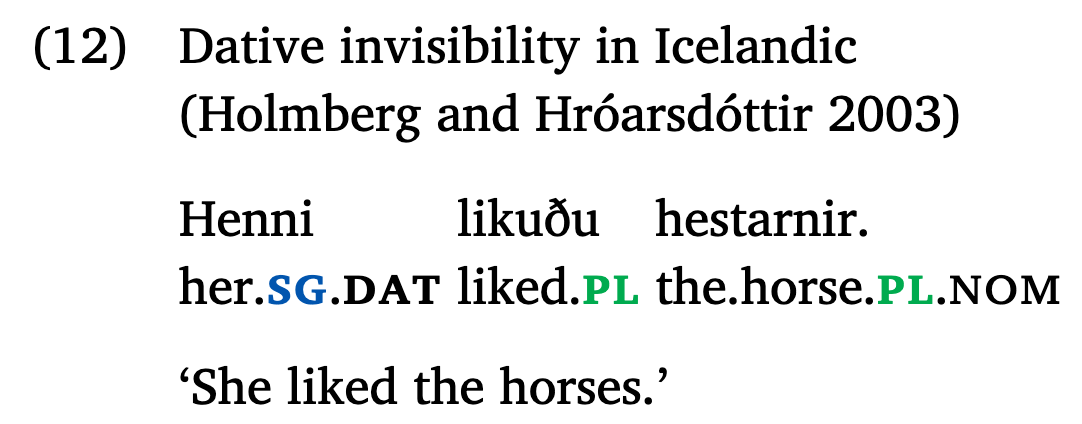
\includegraphics[width=0.52\linewidth]{images/pasted-20260922055800.png}\end{center}

Yes blocking in `transitive expletives' (Holmberg and Hróarsdóttir 2003):

\begin{center}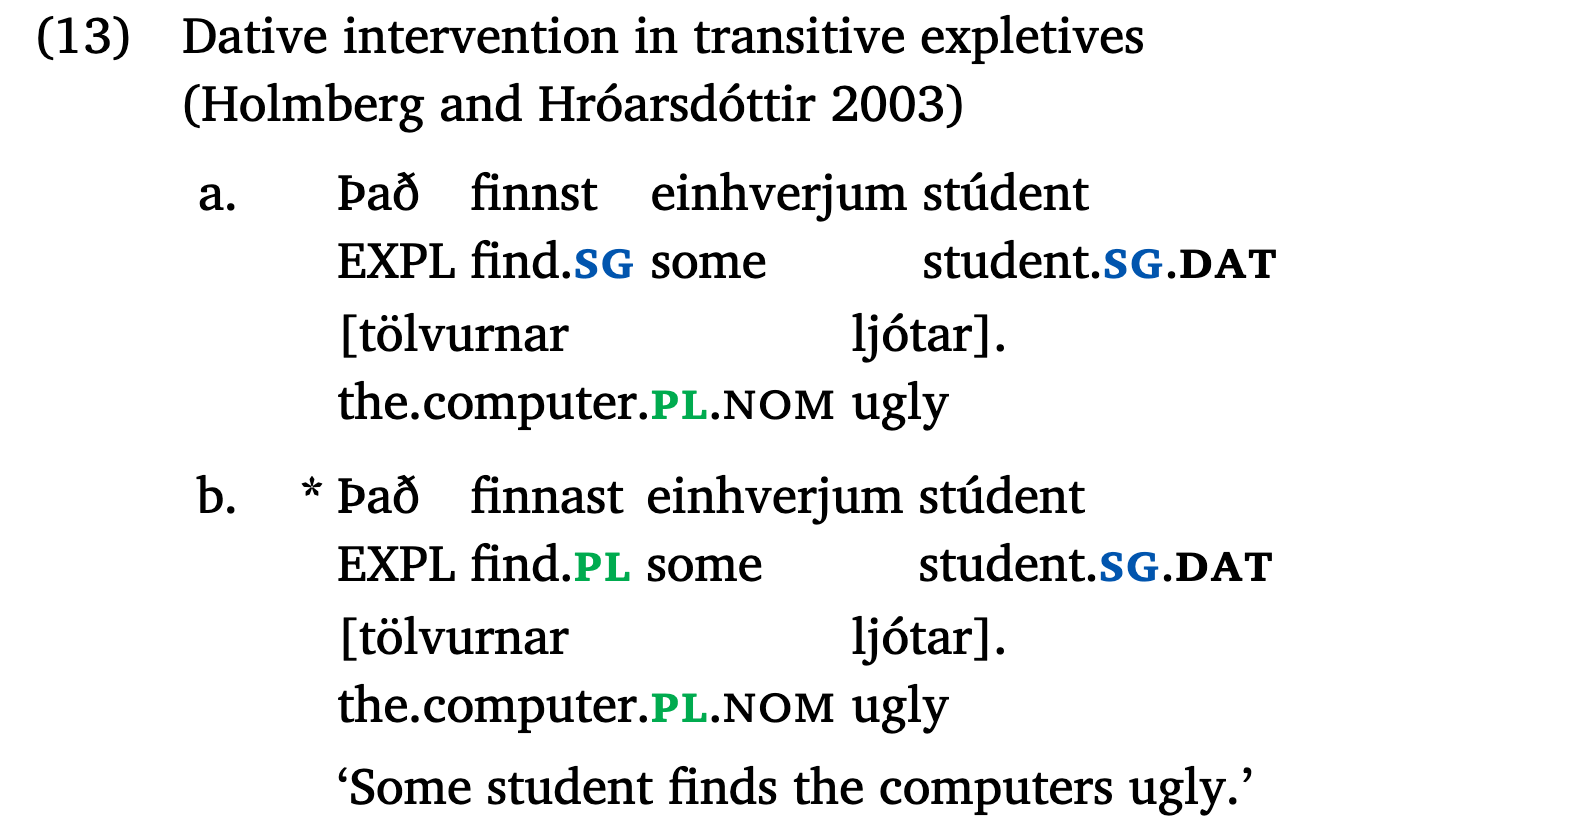
\includegraphics[width=0.58\linewidth]{images/pasted-20260922055807.png}\end{center}

\begin{center}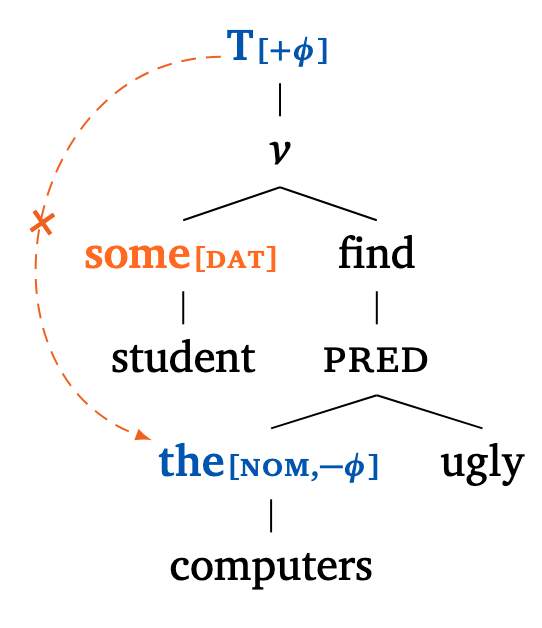
\includegraphics[width=0.26\linewidth]{images/pasted-20260922055815.png}\end{center}

Non-nominative subjects don't agree - usually enforcing agreement with lower nominatives. However, in (13), dative subjects intervene.

\begin{itemize}
  \item The visibility of the dative DP depends partly on whether it undergoes a specific type of movement which is not always available (see later)
  \item also, LDA is subject to dialectal differences and is sometimes optional
\end{itemize}

weird and imo not great solution to this

and then when you raise to specTP:

\begin{center}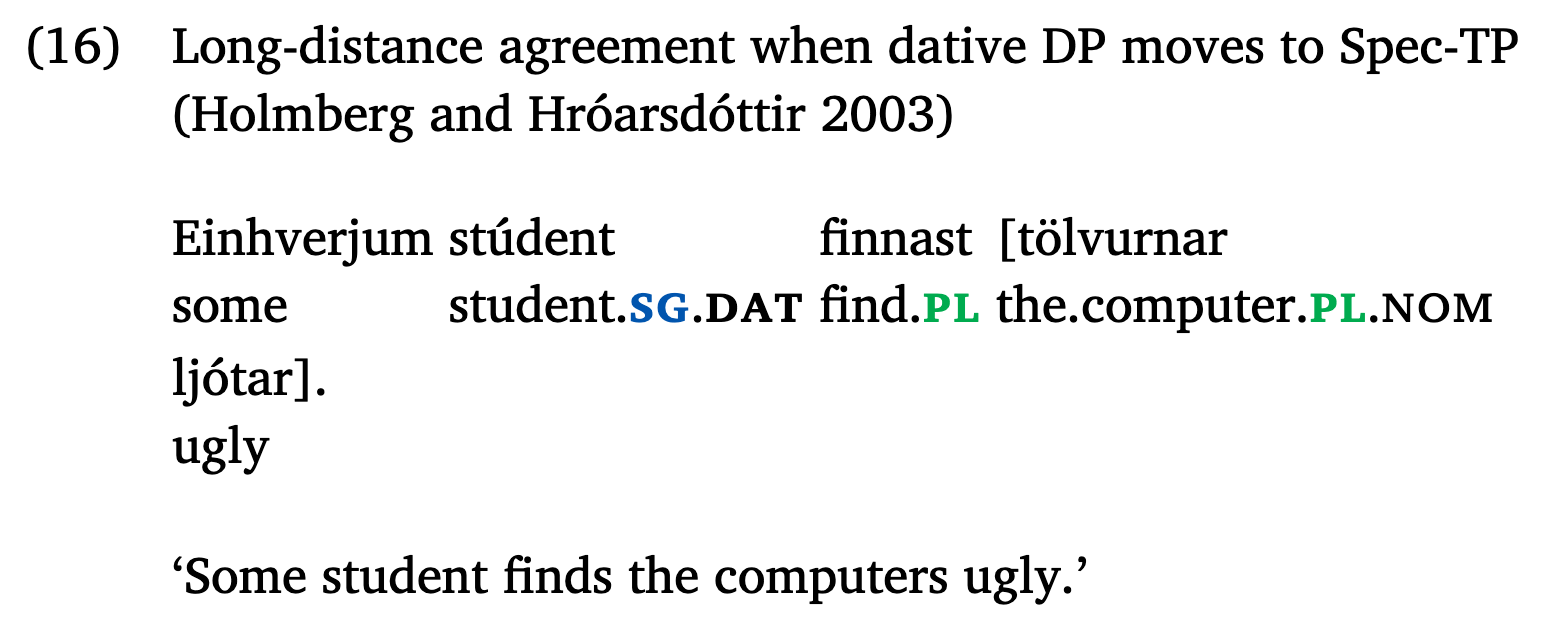
\includegraphics[width=0.56\linewidth]{images/pasted-20260922055826.png}\end{center}

Kenneth: datives are invisible iff they undergo EPP movement

Or: \textbf{project all nominatives, plus datives without EPP}

\subsubsection*{2.2 variation in directionality (Lubukusu: swap phi+ and phi-, agree up)}

Theories:

\begin{itemize}
  \item always downward (Chomsky 2000): goal is below probe
  \item always upward (Zeijlstra 2012)
  \item varies parametrically (Baker 2008)
\end{itemize}

TSL patterns have no fixed directionality so could be both.

\begin{itemize}
  \item in phonology there are both progressive and regressive harmony
\end{itemize}

Subject-Verb agreement is usually downward looking

\begin{itemize}
  \item but Negative Concord is upward looking, plus Case Concord if case goes on D
\end{itemize}

Complementizer Agreement:

\begin{itemize}
  \item West Flemish: complementizer agrees downward for number with embedded subject
  \item Lubukusu: complementizer (sometimes) agrees upward for noun class w higher subject
\end{itemize}

\begin{center}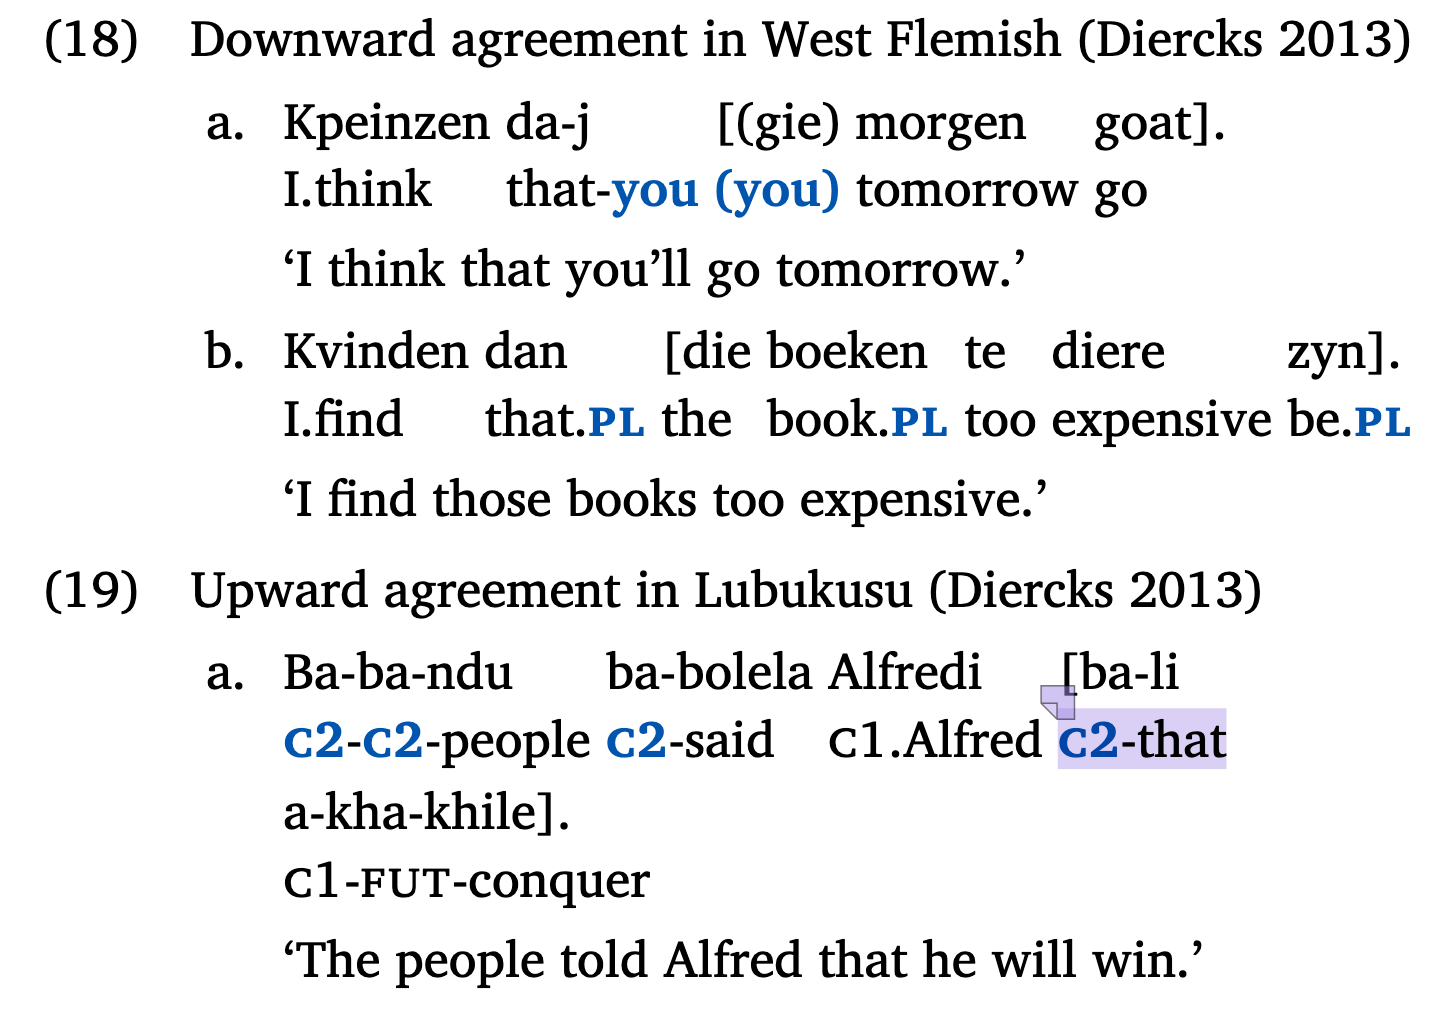
\includegraphics[width=0.61\linewidth]{images/pasted-20260922055842.png}\end{center}

However, Diercks 2013's analysis of Lubukusu:

\begin{itemize}
  \item matrix subject binds an operator in specCP which agrees locally with C
  \item he calls it Indirect Agreement
\end{itemize}
Kenneth has good counters to Dierck's main arguments

\subsubsection*{2.3 multiple probes with single goal (chain agreement: phi+ phi+ ok)}

Don't know cases of (what are phonologically called) Icy Targets in syntax: items which both harmonize and prevent harmony from spreading further

\subsubsection*{2.4 single probe with multiple goals/optionality}

There seem(s) to be some squirrels in the attic.

*Some squirrels seems to be in the attic.

could posit multiple competing grammars (Kroch 1989)

or, single grammar, and Interaction-Satisfaction Theory

\begin{itemize}
  \item for each probe can specify its interaction set (features it agrees with) and satisfaction set (features which cause it to stop)
\end{itemize}
